\documentclass[a4paper, 14pt]{extarticle}
\usepackage{float}
% Поля
%--------------------------------------
\usepackage{geometry}
\geometry{a4paper,tmargin=2cm,bmargin=2cm,lmargin=3cm,rmargin=1cm}
%--------------------------------------


%Russian-specific packages
%--------------------------------------
\usepackage[T2A]{fontenc}
\usepackage[utf8]{inputenc}
\usepackage[english, main=russian]{babel}
%--------------------------------------

\usepackage{textcomp}

% Красная строка
%--------------------------------------
\usepackage{indentfirst}
%--------------------------------------


%Graphics
%--------------------------------------
\usepackage{graphicx}
\graphicspath{ {./images/} }
\usepackage{wrapfig}
%--------------------------------------

% Полуторный интервал
%--------------------------------------
\linespread{1.3}
%--------------------------------------

%Выравнивание и переносы
%--------------------------------------
% Избавляемся от переполнений
\sloppy
% Запрещаем разрыв страницы после первой строки абзаца
\clubpenalty=10000
% Запрещаем разрыв страницы после последней строки абзаца
\widowpenalty=10000
%--------------------------------------

%Списки
\usepackage{enumitem}

%Подписи
\usepackage{caption}

%Гиперссылки
\usepackage{hyperref}

\hypersetup {
	unicode=true
}

%Рисунки
%--------------------------------------
\DeclareCaptionLabelSeparator*{emdash}{~--- }
\captionsetup[figure]{labelsep=emdash,font=onehalfspacing,position=bottom}
%--------------------------------------

\usepackage{tempora}

%Листинги
%--------------------------------------
\usepackage{listings}
\lstset{
  basicstyle=\ttfamily\footnotesize,
  %basicstyle=\footnotesize\AnkaCoder,        % the size of the fonts that are used for the code
  breakatwhitespace=false,        % sets if automatic breaks shoulbd only happen at whitespace
  breaklines=true,                 % sets automatic line breaking
  captionpos=t,                    % sets the caption-position to bottom
  inputencoding=utf8,
  frame=single,                    % adds a frame around the code
  keepspaces=true,                 % keeps spaces in text, useful for keeping indentation of code (possibly needs columns=flexible)
  keywordstyle=\bf,       % keyword style
  numbers=left,                    % where to put the line-numbers; possible values are (none, left, right)
  numbersep=5pt,                   % how far the line-numbers are from the code
  xleftmargin=25pt,
  xrightmargin=25pt,
  showspaces=false,                % show spaces everywhere adding particular underscores; it overrides 'showstringspaces'
  showstringspaces=false,          % underline spaces within strings only
  showtabs=false,                  % show tabs within strings adding particular underscores
  stepnumber=1,                    % the step between two line-numbers. If it's 1, each line will be numbered
  tabsize=2,                       % sets default tabsize to 8 spaces
  title=\lstname                   % show the filename of files included with \lstinputlisting; also try caption instead of title
}
%--------------------------------------

%%% Математические пакеты %%%
%--------------------------------------
\usepackage{amsthm,amsfonts,amsmath,amssymb,amscd}  % Математические дополнения от AMS
\usepackage{mathtools}                              % Добавляет окружение multlined
\usepackage[perpage]{footmisc}
%--------------------------------------

%--------------------------------------
%			НАЧАЛО ДОКУМЕНТА
%--------------------------------------

\begin{document}

%--------------------------------------
%			ТИТУЛЬНЫЙ ЛИСТ
%--------------------------------------
\begin{titlepage}
\thispagestyle{empty}
\newpage


%Шапка титульного листа
%--------------------------------------
\vspace*{-60pt}
\hspace{-65pt}
\begin{minipage}{0.3\textwidth}
\hspace*{-20pt}\centering

\includegraphics[width=\textwidth]{emblem}
\end{minipage}
\begin{minipage}{0.67\textwidth}\small \textbf{
\vspace*{-0.7ex}
\hspace*{-6pt}\centerline{Министерство науки и высшего образования Российской Федерации}
\vspace*{-0.7ex}
\centerline{Федеральное государственное бюджетное образовательное учреждение }
\vspace*{-0.7ex}
\centerline{высшего образования}
\vspace*{-0.7ex}
\centerline{<<Московский государственный технический университет}
\vspace*{-0.7ex}
\centerline{имени Н.Э. Баумана}
\vspace*{-0.7ex}
\centerline{(национальный исследовательский университет)>>}
\vspace*{-0.7ex}
\centerline{(МГТУ им. Н.Э. Баумана)}}
\end{minipage}
%--------------------------------------

%Полосы
%--------------------------------------
\vspace{-25pt}
\hspace{-35pt}\rule{\textwidth}{2.3pt}

\vspace*{-20.3pt}
\hspace{-35pt}\rule{\textwidth}{0.4pt}
%--------------------------------------

\vspace{1.5ex}
\hspace{-35pt} \noindent \small ФАКУЛЬТЕТ\hspace{80pt} <<Информатика и системы управления>>

\vspace*{-16pt}
\hspace{47pt}\rule{0.83\textwidth}{0.4pt}

\vspace{0.5ex}
\hspace{-35pt} \noindent \small КАФЕДРА\hspace{50pt} <<Теоретическая информатика и компьютерные технологии>>

\vspace*{-16pt}
\hspace{30pt}\rule{0.866\textwidth}{0.4pt}

\vspace{11em}

\begin{center}
\Large {\bf Лабораторная работа № 1} \\
\large {\bf по курсу <<Численные методы линейной алгебры>>} \\
\large <<Подготовка вспомогательных средств разработки>>
\end{center}\normalsize

\vspace{8em}


\begin{flushright}
  {Студент группы ИУ9-71Б Баев Д.А \hspace*{15pt}\\
  \vspace{2ex}
  Преподаватель Посевин Д. П.\hspace*{15pt}}
\end{flushright}

\bigskip

\vfill


\begin{center}
\textsl{Москва 2023}
\end{center}
\end{titlepage}
%--------------------------------------
%		КОНЕЦ ТИТУЛЬНОГО ЛИСТА
%--------------------------------------

\renewcommand{\ttdefault}{pcr}

\setlength{\tabcolsep}{3pt}
\newpage
\setcounter{page}{2}

\section{Задание}\label{Sect::task}
1. Подготовить методы для выполнения операций с векторами: вычисление
скалярного произведения двух векторов, вычисление Евклидовой нормы
вектора.

2. Подготовить методы для выполнения операций с матрицами: умножение
матрицы на матрицу, умножение матрицы на вектор, транспонирование
матрицы.

3. Подготовить метод построения графика произвольной функции от одной
переменной.

4. Реализовать оценку погрешности вычисления объема шара зажатого цилиндром тремя способами при двух различных приближениях вычисления значения
\newpage
\section{Исходный код}

Исходный код программы представлен в листингах~\ref{lst:code1}--~\ref{lst:code4}.

\begin{figure}[H]
\begin{lstlisting}[language={},caption={Операции над векторами},label={lst:code1}]
def scalar(vector1, vector2):
    assert len(vector1) == len(vector2)
    return sum(x * y for x, y in zip(vector1, vector2))

def norm(vector):
    return np.sqrt(sum(x**2 for x in vector))

vector1 = [1, 2, 3]
vector2 = [4, 5, 6]

print(scalar(vector1, vector2))
print(norm(vector2))
\end{lstlisting}
\end{figure}

\begin{figure}[H]
\begin{lstlisting}[language={},caption={Операции над матрицами},label={lst:code2}]
def mul_matrix(matrix1, matrix2):
    assert len(matrix1[0]) == len(matrix2)
    return [
        [sum(matrix1[i][k] * matrix2[k][j] for k in range(len(matrix2[0])))
         for j in range(len(matrix2[0]))]
        for i in range(len(matrix1))
    ]

def mul_matrix_by_vector(matrix, vector):
    assert len(matrix[0]) == len(vector)
    return [sum(matrix[i][j] * vector[j] for j in range(len(vector))) for i in range(len(matrix))]

def transpose_matrix(matrix):
    return [list(row) for row in zip(*matrix)]

matrix1 = [[1, 2, 3], [4, 5, 6], [7, 8, 9]]
matrix2 = [[3, 4, 6], [1, 2, 7], [9, 8, 1]]
matrix3 = [[2, 3], [9, 4], [5, 6]]

print(mul_matrix(matrix1, matrix2))
print(mul_matrix_by_vector(matrix1, vector1))
print(transpose_matrix(matrix1))
print(transpose_matrix(matrix3))
\end{lstlisting}
\end{figure}

\begin{figure}[H]
\begin{lstlisting}[language={},caption={Построение графика},label={lst:code3}]
def plot(function, x1, x2, step, x = None):
    x = [x for x in range(x1, x2 + step, step)] if x is None else x
    plt.plot(x, function(np.array(x)))
    plt.show()

def f(x):
    return x**2

plot(f, -10, 10, 1)
\end{lstlisting}
\end{figure}

\begin{figure}[H]
\begin{lstlisting}[language={},caption={Оценка погрешности},label={lst:code4}]
def S1(sqrt):
    return (sqrt - 1) ** 6

def S2(sqrt):
    return (3 - 2 * sqrt) ** 3

def S3(sqrt):
    return 99 - 70 * sqrt

def S1_derivative(sqrt):
    return  6 * (sqrt - 1) ** 5

def S2_derivative(sqrt):
    return -6 * (3 - 2 * sqrt) ** 2

def S3_derivative(sqrt):
    return -70

def V(S):
    return 4/3 * np.pi * S

R = 3

ways = {
    "S1": [S1, S1_derivative],
    "S2": [S2, S2_derivative],
    "S3": [S3, S3_derivative]
}

sqrts = {
    "7/5": 7/5,
    "17/12": 17/12
}

S_list = []
V_list = []
estimation_list = []
for way, func in ways.items():
    for sqrt, value in sqrts.items():
        S = func[0](value)
        V_calc = V(S)
        estimation =  abs(func[1](value) * (value - np.sqrt(2)) / S)
        S_list.append(S)
        V_list.append(V_calc)
        estimation_list.append(estimation * 100)


table = pd.DataFrame(
    {
        "Way": sorted(list(ways.keys()) * 2),
        "Sqrt":  list(sqrts.keys()) * 3,
        "S": S_list,
        "V": V_list,
        "Error estimation": estimation_list
    }
)
print(table)
\end{lstlisting}
\end{figure}

\section{Результаты}

Результат проверки операций над векторами представлен на рисунке~\ref{fig:img1}.

\begin{figure}[H]
\centering
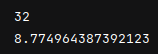
\includegraphics{images/res1.png}
\caption{Результат проверки операций над векторами}
\label{fig:img1}
\end{figure}


Результат проверки операций над матрицами представлен на рисунке~\ref{fig:img2}.


\begin{figure}[H]
\centering
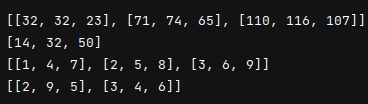
\includegraphics{images/res2.png}
\caption{Результат проверки операций над матрицами}
\label{fig:img2}
\end{figure}


Результат проверки построения графика представлен на рисунке~\ref{fig:img3}.

\begin{figure}[H]
\centering
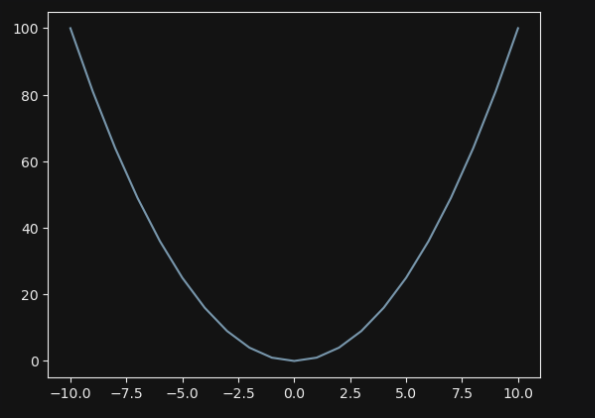
\includegraphics[width=0.8\textwidth]{images/res3.png}
\caption{Результат проверки построения графика}
\label{fig:img3}
\end{figure}


Результат проверки оценки погрешности представлен на рисунке~\ref{fig:img4}.

\begin{figure}[H]
\centering
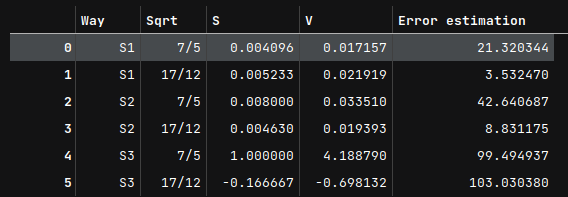
\includegraphics[width=0.8\textwidth]{images/res4.png}
\caption{Результат проверки оценки погрешности}
\label{fig:img4}
\end{figure}

\section{Выводы}
В результате выполнения лабораторной работы были реализованы основные операции с векторами и матрицами, построение графика произвольной функции с помощью Matplotlib, а также метод оценки погрешности вычислений.

Анализируя результат оценки погрешности, можно отметить, что, при разных приближениях данных и при разных, но аналитически тождественных способах вычисления, результат может значительно отличаться.
\end{document}